%
% \iffalse
%<*driver>
\ProvidesFile{nyu22fonts.dtx}[2023/06/13 v0.16a NYU Typefaces and Fonts]
%</driver>
%<pkg>\ProvidesExplPackage{nyu22fonts}{2023/06/13}{v0.16a}{NYU Typefaces and Fonts}
%<*driver>
\documentclass[11pt]{ltxdoc}
\usepackage{dtxdescribe}
\usepackage{graphicx}
\usepackage{changepage}^^A      For the `adjustwidth' environment
\usepackage{hologo}^^A          Provides lots of logos

\usepackage[backend=biber]{biblatex}
\addbibresource{nyu22fonts.bib}

\usepackage{listings}
\lstset{language=bash,basicstyle=\ttfamily}

\usepackage{titling}
\pretitle{\begin{adjustwidth}{0pt}{-1in}\begin{flushleft}\Huge}
\posttitle{\par\end{flushleft}\end{adjustwidth}\vskip 0.5em}
\predate{\begin{flushleft}}
\postdate{\par\end{flushleft}}
\preauthor{\begin{flushleft}}
\postauthor{\par\end{flushleft}}

\usepackage{xcolor-nyu22}[2022/08/05]
\colorlet{\watchoutcolor}{Magenta}
\usepackage[Gotham, Frank Ruhl Libre]{nyu22fonts}
\linespread{1.041667}
\setmonofont{Inconsolata}

% For documenting expl3 macros, surround the doc element with |\makeusletter|
% and |\makeussubscript|.
\newcommand{\makeusletter}{\catcode`\_=12}
\newcommand{\makeussubscript}{\catcode`\_=8}



% In the contemporary/subtle tone quadrant, we use sans for the main text and
% serif for the section titles.
%
% These font assignments have nothing to do with this package; they are part of
% the styling of a document.
\renewcommand{\familydefault}{\sfdefault}
\usepackage{titlesec}
\newcommand{\headingfont}{\rmfamily\color{NyuViolet}}
\titleformat*{\section}{\LARGE\headingfont}
\titleformat*{\subsection}{\Large\headingfont}
\titleformat*{\subsubsection}{\large\headingfont}
\renewcommand{\maketitlehooka}{\headingfont}

\usepackage{parskip}

\EnableCrossrefs
\RecordChanges
\CodelineIndex
\usepackage{hyperref}
\AtBeginDocument{
  \hypersetup{
    allcolors=NyuViolet,
  }
}
\begin{document}
  \DocInput{nyu22fonts.dtx}
\end{document}
%</driver>
% \fi

% \GetFileInfo{nyu22fonts.dtx} 
% \title{NYU Typefaces and Fonts}
% \author{Matthew Leingang\thanks{leingang@nyu.edu}} \date{\fileversion, Released \filedate}
% \maketitle

% \begin{abstract}
%  This package will load fonts for the NYU brand.
%  Package options will allow choices among the primary (proprietary) faces,
%  open (Google) faces, system (Microsoft) faces, and T1 fonts for those who
%  must use \texttt{pdftex}. 
% \end{abstract}

% \changes{0.10.4}{2019/12/10}{First working release}
% \changes{0.11.0}{2022/08/16}{Full Implementation of package options}

% \section{Introduction}

% \subsection{The NYU Typographic Style}
%
% \begin{quotation}
% NYU's typographic language brings your communication to life. Like color, the
% fonts we use reinforce the tone of our communications and designs.
%
% Gotham and Mercury Text are NYU's two typefaces. [See Figures
% \ref{fig-gotham}~and~\ref{fig-mercury-text}.] This versatile group of font
% families can be combined to achieve different tones. That flexibility helps
% our communications appeal to many of our different audiences, including
% students, parents, alumni, faculty and staff, peers, and supporters, while
% maintaining a thematically consistent brand. Font choice also establishes a
% clear hierarchy of information, allowing audiences to easily navigate your
% communications.
%
% \textbf{Gotham} references the no-nonsense signage of New York City. It's a
% typeface that's meant to feel familiar and approachable but strong enough to
% grab and hold your attention within the busy city.
%
% \textbf{Mercury Text} is a high performance serif typeface born from nearly a
% decade of research and development. Mercury Text is resilient enough to work
% in a wide variety of communications.
%
% \hfill---NYU Media and Communications~\cite{nyu-fonts}
% \end{quotation}
%
% \begin{figure}
% 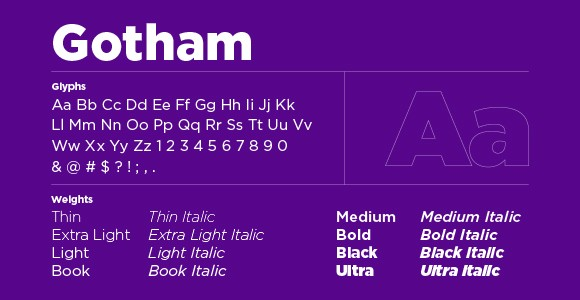
\includegraphics[width=\textwidth]{1645638294211}
% \caption{Gotham and its weights (from~\cite{nyu-fonts})}
% \label{fig-gotham}
% \end{figure}
%
% \begin{figure}
% 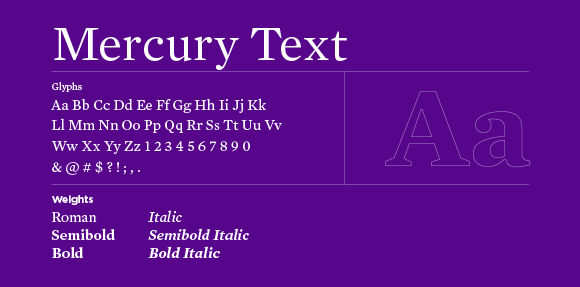
\includegraphics[width=\textwidth]{1645638337298}
% \caption{Mercury Text and its weights (from~\cite{nyu-fonts})}
% \label{fig-mercury-text}
% \end{figure}
%
% \subsection{Engines and Font Encodings}
%
% There are several ways a font can be encoded. The ``old'' format is
% PostScript Type~1 or just ``T1''.~\cite{enwiki:1104696616}.  The old format
% is not \emph{as} old as \hologo{TeX}'s native font file format.  Ironically,
% the method for selecting Type~1 fonts in \hologo{TeX} is called the NFSS or
% ``new font selection scheme.''~\cite{texdoc-fntguide}
%
% The ``new'' (still quite old, late 1980s) formats are TrueType (see
% \cite{enwiki:1092758383}) and OpenType. OpenType was built onto TrueType and
% was released in 1996.
%
% There are also several programs, called \emph{engines}, which convert a
% \filenm{.tex} file to a PDF.
%
% Most of the time, the default engine is \hologo{pdfTeX}. This engine only
% handles Type~1 fonts, however. The 21st century engines were designed to
% handle OpenType and TrueType fonts.  \hologo{XeTeX} (first released in 2004)
% also reads input files in unicode rather than plain ASCII, and
% \hologo{LuaTeX} (since 2007) includes a scriptable layer in the lua language.
% The \pkg{fontspec} package~\cite{pkg-fontspec} provides a more modern font
% specification interface.
%
% The upshot is that \textbf{if you want the full features of this package, you
% must use \hologo{XeLaTeX} or \hologo{LuaLaTeX}}. But there are other reasons
% to use them, anyway.  \hologo{LuaTeX} is the engine most in active
% development, so that is the recommended modern engine to adapt.
%
% If you typeset your \filenm{.tex} files on the command line, you just type
% \prog{lualatex} instead of \prog{latex} or \prog{pdflatex}. If you use
% some kind of GUI editor with \hologo{LaTeX} features, search its documentation
% for ``engine'' and you will probably find the option to configure it.

% \section{Installation}

% \subsection{The package}

% To install the package, download the repository and within the module directory,
% execute the command: \prog{l3build install}.

% \subsection{The fonts}
%
% \subsubsection{Gotham}
% 
% To install Gotham, go to \href{https://nyu.onthehub.com/}{OnTheHub} and download
% the zip file of TrueType fonts. Then open the archive and double click on each font.
% It should be added to your system's font library.
%
% \subsubsection{Mercury Text}
%
% To install Mercury text, you would need to purchase it directly from
% \href{https://www.typography.com/fonts/mercury-text/styles}{Hoefler\&Co}. 
%
% There \watchout[warning] are pirated TrueType font files purporting to 
% provide various grades of Mercury Text, but they are incorrectly encoded.
% The letters are fine, but several punctuation glyphs are given the wrong
% unicode point. If you install them, your text will be missing quotation marks
% and other punctuation. If you don't want to pay big bucks for Mercury Text,
% settle for Frank Ruhl Libre.
% 
% \subsubsection{Montserrat}
%
% \begin{figure}
% 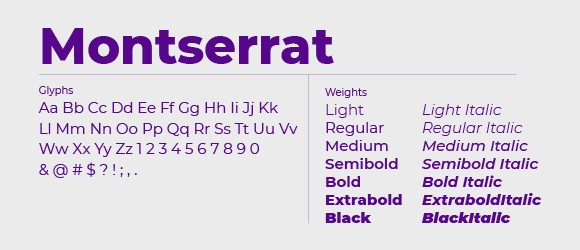
\includegraphics[width=\textwidth]{1645638304749}
% \caption{Montserrat and its weights (from~\cite{nyu-fonts})}
% \label{fig-montserrat}
% \end{figure}
% Montserrat (see Figure~\ref{fig-montserrat}) is a TrueType font that is
% included in \hologo{TeX}~Live. So you won't need to install it separately.
%
% \subsubsection{Frank Ruhl Libre}
% 
% \begin{figure}
% 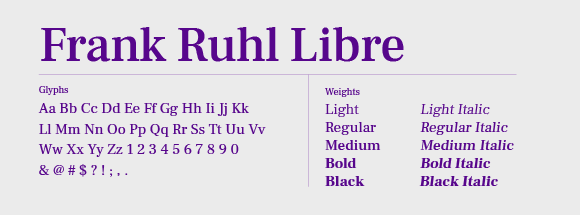
\includegraphics[width=\textwidth]{1645638347113}
% \caption{Frank Ruhl Libre and its weights (from~\cite{nyu-fonts})}
% \label{fig-frl}
% \end{figure}
%
% Frank Ruhl Libre (see Figure~\ref{fig-frl}) is an open licensed TrueType
% font, but it's not in \hologo{TeX}~Live. You can download it from
% \href{https://fonts.google.com/specimen/Frank+Ruhl+Libre}{Google Fonts}.
% Install it by opening the zip file and double-clicking.
%
% \subsubsection{Other Fonts}
%
% The remaining TrueType fonts referenced in this package (Helvetica, Arial,
% Georgia, Times New Roman) should be on your machine already if you have any
% Microsoft or Apple product installed.
%
% The Type~1 fonts referenced will be in \hologo{TeX}~Live.
%
% \section{Usage}
%
% Almost everything in the package is described with keys, as in PGF/TikZ.
% For example:
% \begin{sourcedisplay}
% \cs{usepackage}\oarg{keyvals}\{nyu22fonts\}
% \end{sourcedisplay}
%
% \DescribeMacro{\nyufontssetup}\marg{keyvals}
% 
% Configure package options after loading, if possible. Options which require loading additional packages
% can only be used in the preamble.
%
% \subsection{\hologo{XeLaTeX} and \hologo{LuaLaTeX} usage}
%
% With either of the engines that support TrueType fonts, we can use those
% fonts.
% 
% \subsubsection{Setting fonts in groups}
%
% \begin{description}
%
%   \ItemDescribeKey{proprietary} Load Gotham and Mercury Text.
%
%   This option can't be used unless you have \textbf{both}
%   Gotham and Mercury Text. \watchout
%
%   \ItemDescribeKey{open} Load Montserrat and Frank Ruhl Libre.  
%
%   \ItemDescribeKey{system} Load Helvetica and Times New Roman.
%
% \end{description}
%
% \subsubsection{Setting fonts by name}
%
% \begin{description}
%   \ItemDescribeKey{Gotham} Use the Gotham family of fonts.
%     To be more precise, this sets:
%     \begin{itemize}
%        \item the default sans font to Gotham Book
%        \item the default bold sans font to Gotham Medium
%        \item the default italic sans font to Gotham Book Italic
%     \end{itemize}
%
%  \ItemDescribeKey{Mercury Text} Use the Mercury Text G2 family of fonts.
%
%  \ItemDescribeKey{Montserrat} Use the Montserrat family of fonts.
%    As of now, this sets:
%    \begin{itemize}
%      \item the default sans font to Montserrat Regular
%      \item the default bold sans font to Montserrat Bold
%      \item the default italic sans font to Montserrat Italic
%    \end{itemize}
%    This may change in the future, since, like Gotham, Montserrat comes
%    in a variety of weights.
%
%  \ItemDescribeKey{Helvetica} Use the Helvetica TrueType family of fonts.
%
%  \ItemDescribeKey{Times New Roman} Use the Times New Roman TrueType family
%    of fonts.
% 
% \end{description}
%
% \subsubsection{Setting fonts automatically}
%
% \DescribeKey{auto}
% Choose the ``best'' available sans and serif fonts. The order of preference
% is proprietary (i.e., Gotham and Mercury Text), open licensed fonts (i.e., 
% Montserrat and Frank Ruhl), then system fonts (i.e., Helvetica and Times New
% Roman). Each font is chosen independently, so you can end up with (for 
% instance) Gotham and Frank Ruhl Libre. 
%
% Use this option with care, because it searches the file system for fonts at
% each \LaTeX{} run. This can slow down your workflow quite a bit.
%
% \subsection{\hologo{pdfLaTeX} usage}
%
% With the \hologo{pdfLaTeX} engine, a reasonable attempt is made to imitate
% the desired fonts with available Type~1 alternatives.
%
% \begin{description}
%
%   \ItemDescribeKey{open} Load Vera Sans and Bitstream Charter.  These are
%     decent Type~1 alternatives to Gotham and Mercury Text.
%
%   \ItemDescribeKey{system} Load Type~1 versions of Helvetica and Times New
%     Roman. 
%
% \end{description}
%
% Setting |proprietary| with this engine will \watchout[unavailable key]
% issue a warning, since the proprietary fonts are not available. As a
% fallback, the |system| key is set instead.
%
%
% \StopEventually{\PrintChanges}
%
% \printbibliography
%
% \section{Implementation}
% \makeusletter
%    \begin{macrocode}
%<*pkg>
%    \end{macrocode}
%
% Can we use \texttt{fontspec}?
% If so, load it.
%    \begin{macrocode}
\bool_new:N \l_nyu_fontspec_bool
\bool_set_false:N \l_nyu_fontspec_bool
\sys_if_engine_luatex:T { \bool_set_true:N \l_nyu_fontspec_bool }
\sys_if_engine_xetex:T  { \bool_set_true:N \l_nyu_fontspec_bool }

\bool_if:NT \l_nyu_fontspec_bool { \RequirePackage{fontspec}}

\msg_new:nnnn { nyu22fonts } { needsfontspec }{
  Option~`#1'~requires~xelatex~or~lualatex.
}{
  The~option~`#1'~requires~the~xetex~or~luatex~engines~and~
  cannot~be~used~with~pdftex.
}
\msg_new:nnn { nyu22fonts }{ missingssfont }{
  No~sans~serif~font~found.
}
\msg_new:nnn { nyu22fonts }{ missingsffont }{
  No~serif~font~found.
}
%    \end{macrocode}
%
%
% \subsection{Font specification commands}
%
% \subsubsection{Proprietary fonts}
%
% \begin{macro}{\l_nyu_set_gotham:}
% Set the default sans family to Gotham.
%    \begin{macrocode}
\cs_new:Nn \l_nyu_set_gotham: {
  \setsansfont{Gotham}[
    UprightFont=*~Book,
    BoldFont=*~Medium,
    ItalicFont=*~Book~Italic
  ]          
}
%    \end{macrocode}  
% \end{macro}
%
% \begin{macro}{\l_nyu_set_mercury_text:}
% Set the default roman family to Mercury Text Grade~2.
%    \begin{macrocode}
\cs_new:Nn \l_nyu_set_mercury_text: {
  \setmainfont{Mercury~Text~G2}[
    UprightFont=*~Roman,
    BoldFont=*~Bold,
    ItalicFont=*~Italic
  ]
}
%    \end{macrocode}  
% \end{macro}
%
% \subsubsection{Open fonts}
%
% \begin{macro}{\l_nyu_set_montserrat:}
% Set the default sans family to Montserrat. There is already a
% \pkg{montserrat} package with a \filenm{montserrat.fontspec} file, so we just
% have to load it.
%    \begin{macrocode}
\cs_new:Nn \l_nyu_set_montserrat: {
  \setsansfont{montserrat}
}
%    \end{macrocode}
% \end{macro}
%
% \begin{macro}{\l_nyu_set_frank_ruhl_libre:}
% Set the default roman family to Frank Ruhl Libre. 
% \changes{v0.14h}{2023/06/12}{Don't also set the sans font simultaneously.}
%    \begin{macrocode}
\cs_new:Nn \l_nyu_set_frank_ruhl_libre: {
  \setmainfont{Frank~Ruhl~Libre}[
    ItalicFont=*,
    ItalicFeatures={FakeSlant}
  ]
}
%    \end{macrocode}
% \end{macro}
%
% \subsubsection{\LaTeX{} Type~1 approximations}
% 
% These are not official font options but pretty good approximations to
% the official open ones.
% 
% \begin{macro}{\l_nyu_set_vera:}
% Set the default sans family to Vera. The mono family is set to Bera, 
% but the roman family is left alone.
% \changes{v0.11c}{2022/10/01}{Fix a bug introduced by the \pkg{arev} package also setting the \emph{serif} font.}
%    \begin{macrocode}
\cs_new:Nn \l_nyu_set_vera: {
  \RequirePackage[T1]{fontenc}
  \RequirePackage{textcomp}
  \renewcommand{\sfdefault}{fav}
  \renewcommand{\ttdefault}{fvm}
  \RequirePackage{arevmath}
  \RequirePackage{beramono}
}
%    \end{macrocode}  
% \end{macro}
%
% \begin{macro}{\l_nyu_set_charter:}
% Set the default roman family to Charter.
%    \begin{macrocode}
\cs_new:Nn \l_nyu_set_charter: {
  \RequirePackage{charter}
}
%    \end{macrocode}  
% \end{macro}
%
%
% \subsubsection{System Fonts}
%
% \begin{macro}{\l_nyu_set_helvetica_tt:}
% Set the default sans family to the TrueType Helvetica font.
%    \begin{macrocode}
\cs_new:Nn \l_nyu_set_helvetica_tt: {
  \setsansfont{Helvetica}
}
%    \end{macrocode}
% \end{macro}
%
% \begin{macro}{\l_nyu_set_times_new_roman_tt:}
% Set the default roman family to the TrueType Times New Roman font.
%    \begin{macrocode}
\cs_new:Nn \l_nyu_set_times_new_roman_tt: {
  \setmainfont{Times~New~Roman}
}
%    \end{macrocode}
% \end{macro}
%
% \subsubsection{Type 1 fonts}
%
% \begin{macro}{\l_nyu_set_helvetica_ti:}
% Set the default sans family to the Type~1 version of Helvetica.
% (Technically, not Helvetica, but a Type~1 clone called Nimbus Sans.)
%    \begin{macrocode}
\cs_new:Nn \l_nyu_set_helvetica_ti: {
  \usepackage{helvet}
}
%    \end{macrocode}
% \end{macro}
%
% \begin{macro}{\l_nyu_set_times_new_roman_ti:}
% Set the default roman family to the Type~1 version of Times New Roman.
%    \begin{macrocode}
\cs_new:Nn \l_nyu_set_times_new_roman_ti: {
  \usepackage{mathptmx}
}
%    \end{macrocode}
% \end{macro}
%
%  
% \subsection{Selecting fonts automatically}
%
% \begin{macro}{\l_nyu_auto_select_ss_font:}
% Choose the sans serif font automatically.
%    \begin{macrocode}
\cs_new:Nn \l_nyu_auto_select_ss_font: {
  \bool_if:NTF \l_nyu_fontspec_bool {
    \fontspec_font_if_exist:nTF { Gotham~Book } {
      \l_nyu_set_gotham:
    }{
      \fontspec_font_if_exist:nTF { Montserrat } {
        \l_nyu_set_montserrat:
      }{
        \fontspec_font_if_exist:nTF { Helvetica } {
          \l_nyu_set_helvetica_tt:
        }{
          \msg_error:nn { nyu22fonts }{ missingssfont }
        }
      }
    }
  }{
    \l_nyu_set_vera:
  }
}
%    \end{macrocode}
% \end{macro}
%
% \begin{macro}{\l_nyu_auto_select_sf_font:}
% Choose the serif font automatically.
%    \begin{macrocode}
\cs_new:Nn \l_nyu_auto_select_sf_font: {
  \bool_if:NTF \l_nyu_fontspec_bool {
    \fontspec_font_if_exist:nTF { Mercury~Text~G2~Roman } {
      \l_nyu_set_mercury_text:
    }{
      \fontspec_font_if_exist:nTF { Frank~Ruhl~Libre } {
        \l_nyu_set_frank_ruhl_libre:
      }{
        \fontspec_font_if_exist:nTF { Times~New~Roman } {
          \l_nyu_set_helvetica_tt:
        }{
          \msg_error:nn { nyu22fonts }{ missingsffont }
        }
      }
    }
  }{
    \l_nyu_set_charter:
  }
}
%    \end{macrocode}  
% \end{macro}

% \section{Keyval interface}
%
% The main processing is done with a keyval interface.
% \changes{v0.15}
%  {2023/06/12}
%  {Fix a bug wherein spaces in option values were ignored}
%    \begin{macrocode}
\keys_define:nn { nyufonts }
  {
    proprietary .meta:n = { font-group = proprietary },
    open .meta:n = { font-group = open },
    system .meta:n = { font-group = system},
    auto .code:n = { 
      \l_nyu_auto_select_sf_font:
      \l_nyu_auto_select_ss_font:
    },

    serif-font .choice:,
    serif-font / Mercury~Text           .code:n = { \l_nyu_set_mercury_text: },
    serif-font / Frank~Ruhl~Libre       .code:n = { \l_nyu_set_frank_ruhl_libre:}, 
    serif-font / Charter                .code:n = { \l_nyu_set_charter:},
    serif-font / Charter                .usage:n = preamble,
    serif-font / Times~New~Roman~Type~1 .code:n = { \l_nyu_set_times_new_roman_ti: },
    serif-font / Times~New~Roman~Type~1 .usage:n = preamble,
    serif-font / Times~New~Roman~TrueType .code:n = { \l_nyu_set_times_new_roman_tt: },

    sans-serif-font .choice:,
    sans-serif-font / Gotham           .code:n = { \l_nyu_set_gotham: },
    sans-serif-font / Montserrat       .code:n = { \l_nyu_set_montserrat: },
    sans-serif-font / Helvetica~Type~1 .code:n = { \l_nyu_set_helvetica_ti: },
    sans-serif-font / Helvetica~Type~1 .usage:n = preamble,
    sans-serif-font / Helvetica~TrueType .code:n = {\l_nyu_set_helvetica_tt: },
    sans-serif-font / Vera             .code:n = { \l_nyu_set_vera: },
    sans-serif-font / Vera             .usage:n = preamble,
%    \end{macrocode}
%
% \begin{key}{Gotham}
% \changes{v0.14h}{2023/06/12}{Added Gotham and Frank Ruhl Libre meta-keys}
% Set Gotham.
%    \begin{macrocode}
    Gotham .meta:n = { sans-serif-font = Gotham }, 
%    \end{macrocode}
% \end{key}
% \begin{key}{Frank Ruhl Libre}
% Set Frank Ruhl Libre.
%    \begin{macrocode}
    Frank~Ruhl~Libre .meta:n = { serif-font = Frank~Ruhl~Libre },
%    \end{macrocode}
% \end{key}  
%
% \changes{v0.16}{2023/06/12}{Added the rest of the TrueType fonts as meta-keys}
%    \begin{macrocode}
    Montserrat .meta:n = { sans-serif-font = Montserrat }, 
    Helvetica .meta:n = { sans-serif-font = Helvetica~TrueType }, 

    Mercury~Text .meta:n = { serif-font = Mercury~Text},
    Times~New~Roman .meta:n = { serif-font = Times~New~Roman~TrueType},


 
    font-group .choice:,
    font-group / proprietary .code:n = {
      \bool_if:NTF \l_nyu_fontspec_bool {
        \l_nyu_set_gotham:
        \l_nyu_set_mercury_text:
      }{
        \msg_error:nnn { nyu22fonts } { needsfontspec } { proprietary }
        \l_nyu_set_helvetica_ti:
        \l_nyu_set_times_new_roman_ti:
      }
    },
    font-group / open .code:n = {
      \bool_if:NTF \l_nyu_fontspec_bool {
        \l_nyu_set_montserrat:
        \l_nyu_set_frank_ruhl_libre:
      }{
        \l_nyu_set_vera:
        \l_nyu_set_charter:
      }
    },
    font-group / system .code:n = {
      \bool_if:NTF \l_nyu_fontspec_bool {
        \l_nyu_set_helvetica_tt:
        \l_nyu_set_times_new_roman_tt:
      }{
        \l_nyu_set_helvetica_ti:
        \l_nyu_set_times_new_roman_ti:
      }
    },
    font-group .initial:n = system,
  }
%    \end{macrocode}
% \makeussubscript
%
% Process keyval options provided with \cs{usepackage}.
% The \pkg{l3keys2e} package is obsolete with the June 2022 \LaTeX{} release.
% See~\cite{tse-l3keys2e}.
%    \begin{macrocode}
\IfFormatAtLeastTF { 2022-06-01 }
{ 
  \ProcessKeyOptions [ nyufonts ]
}{
  \RequirePackage { l3keys2e }
  \ProcessKeysOptions { nyufonts }
}  
%
%    \end{macrocode}
%
% \begin{macro}{\nyufontssetup}
% Set keyval options after package loading.
%    \begin{macrocode}
\newcommand{\nyufontssetup}[1]{
  \IfFormatAtLeastTF { 2022-06-01 }
  { 
    \SetKeys[ nyufonts ]{#1} 
  }{  
    \keys_set:nn { nyufonts }{ #1 } 
  }  
}
%    \end{macrocode}
% \end{macro}
%
%    \begin{macrocode}
%</pkg>
%    \end{macrocode}
%
% \Finale
%
